%! TEX root = analisis_sirkulasi_temu10.tex
% the main TeX file which is intended to compile, :VimtexReload after adjustment
% :h vimtex-tex-root
\documentclass[../main.tex]{subfiles}
% \includeonlyframes{current}
% \setbeameroption{hide notes} % Only slides
% \setbeameroption{show only notes} % Only notes
% \setbeameroption{show notes on second screen=right} % Both

\begin{document}

\bgdarkimg{sirkulasi_0}
\bgdarkimg{sirkulasi_01}

\begin{frame}[mytitle=standard,c,mycolor=digiPH_creamy,dark]
	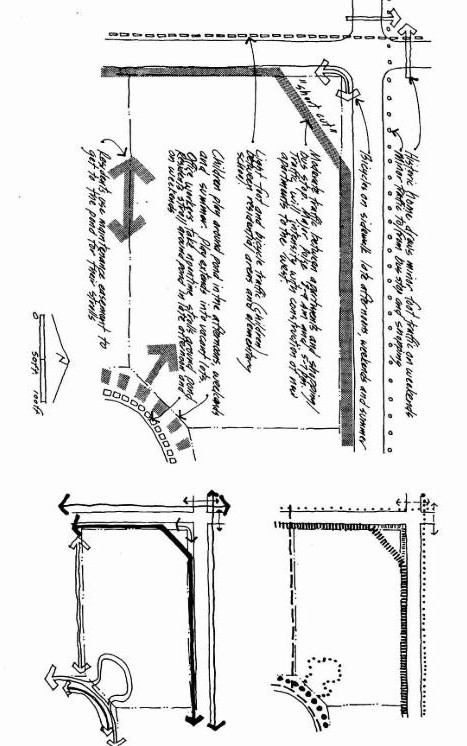
\includegraphics[width=.7\textwidth, angle=90]{../figures/sirkulasi_1}
\end{frame}
\begin{frame}[mytitle=standard,c,mycolor=digiPH_creamy,dark]
	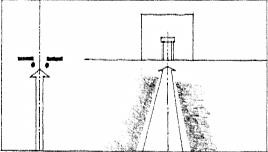
\includegraphics[width=.7\textwidth]{../figures/sirkulasi_2}
\end{frame}

\begin{frame}[mytitle=standard,c,mycolor=digiPH_creamy,dark]
	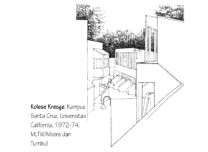
\includegraphics[width=.4\textwidth]{../figures/sirkulasi_3}
\end{frame}

\begin{frame}[mytitle=standard,c,mycolor=digiPH_creamy,dark]
	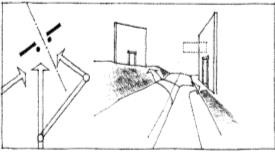
\includegraphics[width=.4\textwidth]{../figures/sirkulasi_4}
\end{frame}

\begin{frame}[mytitle=standard,c,mycolor=digiPH_creamy,dark]
	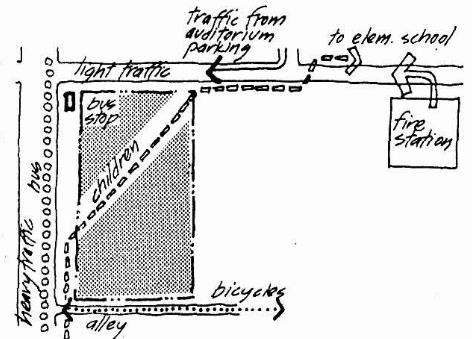
\includegraphics[width=.7\textwidth]{../figures/sirkulasi_5}
\end{frame}

\begin{frame}[mytitle=standard,c,mycolor=digiPH_creamy,dark]
	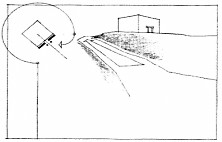
\includegraphics[width=.4\textwidth]{../figures/sirkulasi_6}
\end{frame}

\begin{frame}[mytitle=standard,c,mycolor=digiPH_creamy,dark]
	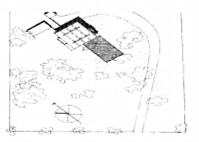
\includegraphics[width=.4\textwidth]{../figures/sirkulasi_7}
\end{frame}
\bgdarkimg{sirkulasi_8}

\bgdarkimg{semua_2_cth}

\begin{frame}[mytitle=standard,c,mycolor=digiPH_creamy,dark]
	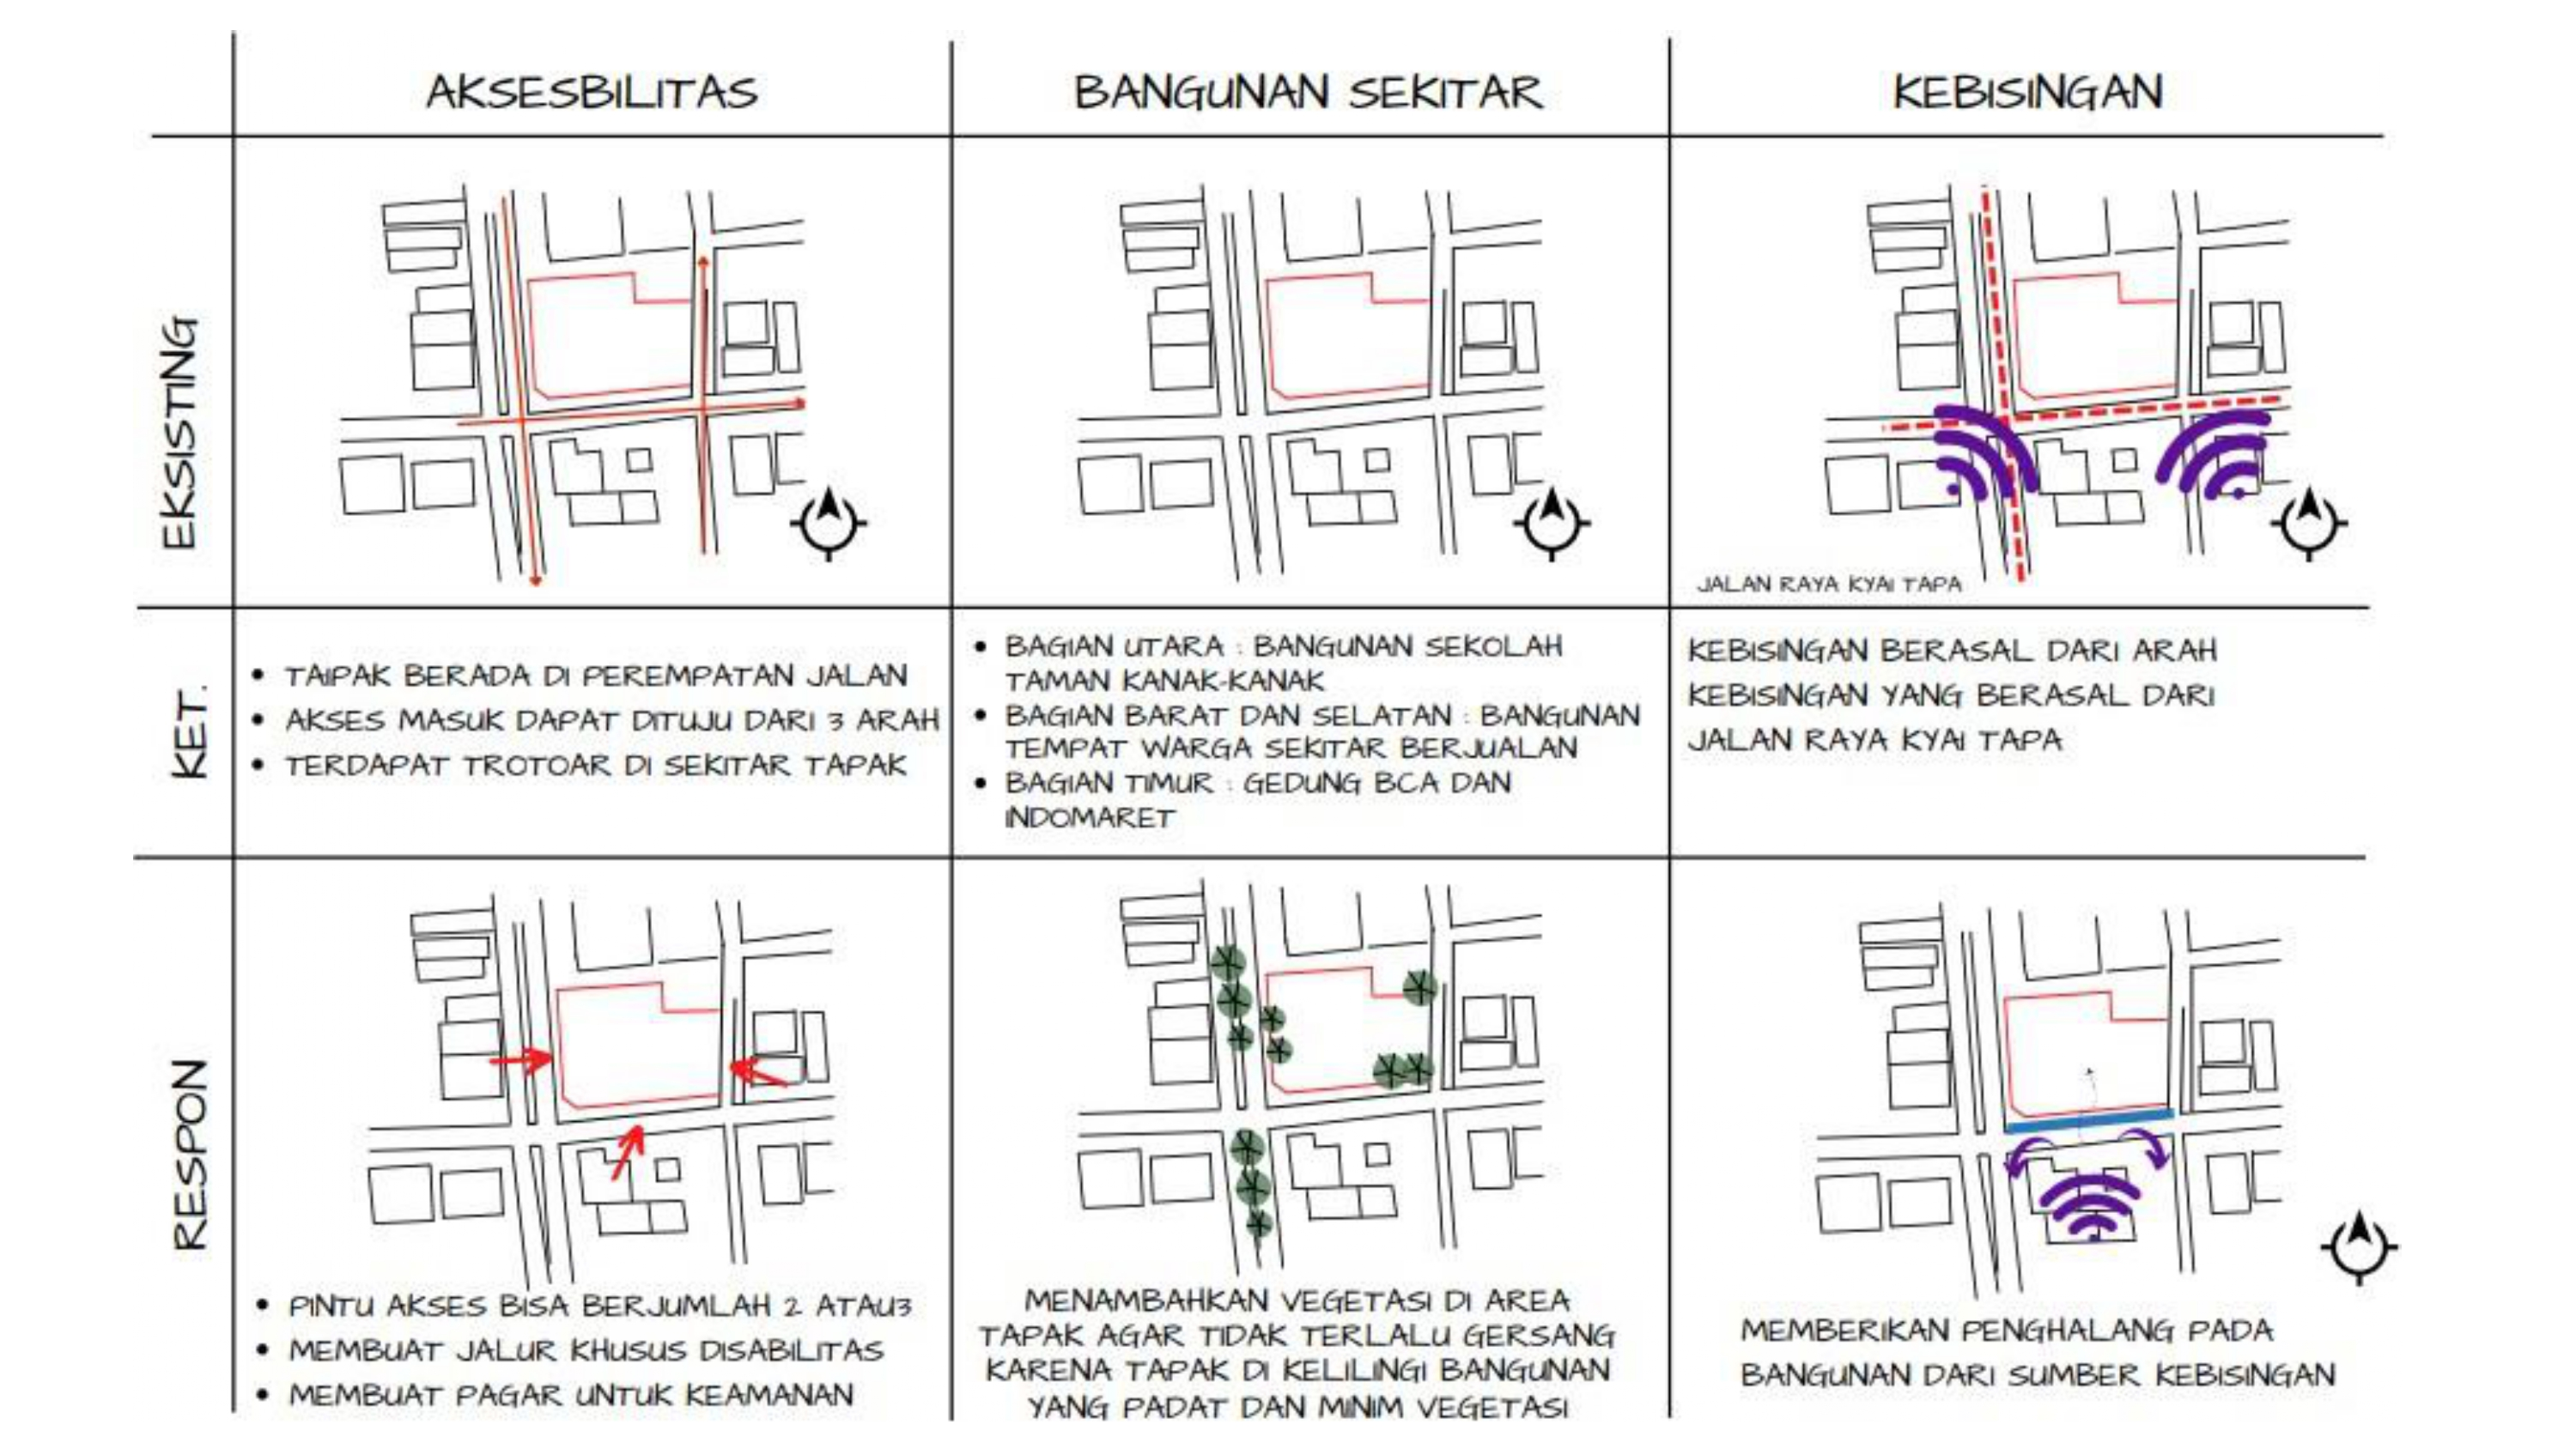
\includegraphics[width=.9\textwidth]{../figures/akses_lingkungan_bising_cth}
\end{frame}

\bgdarkimg{sirkulasi}



\end{document}
